\clearpage
\section{Experimentación Y Resultados}

\subsection{Introducción}
 Realizamos los experimentos en tres computadoras con procesadores similares y se trató de mantener cualquier otro programa cerrado. Igualmente cada conjunto de test fue resuelto en la misma máquina para que las diferencias sean lo más dependendientes a los inputs y los procesos posible.

\subsection{Temperatura en el punto crítico variando granularidad}

En esta sección queremos ver que ocurre con la temperatura en el punto crítico para distintas granularidades de la misma instancia. Para tal fin vamos a presentar distintos tipos de instancias que pueden ser enriquecedoras para el analisis. Queremos aclarar que no nos pareció relevante el analisis con un sanguijuela sobre el punto crítico ya que la temperatura no sufriría variación alguna. Esto último es debido a que todavía no utilizaremos los metodos de eliminación de sanguijuelas para mantener el punto crítico a menos de 235º

\begin{description}

\item[Caso 1:] 8 sanguijuelas rodeando al punto crítico.
\item[Caso 2:] Una sanguijuela muy cercana al punto crítico.
\item[Caso 3:] 5 sanguijuelas alineadas debajo del punto crítico.
\end{description}

Las condiciones del parabrisas que utilizaremos para los 5 casos seran similiares, un ancho y alto de 1024 (para tener un gran espacio de testeo y cantidad de divisores), con una temperatura de 400º para las sanguijuelas (para que influya pero que a su vez no sean tan determinantes) y un radio de 16 posiciones. El valor de las discretizaciones que elegimos para cada caso está limitado en función la cantidad de sanguijuelas ya que a medida que aumenta el valor la cantidad de posiciones disponibles en el parabrisas disminuye\\ \\
\newpage
Caso 1:

\begin{figure}[htb]
\minipage{0.5\textwidth}
\begin{center}
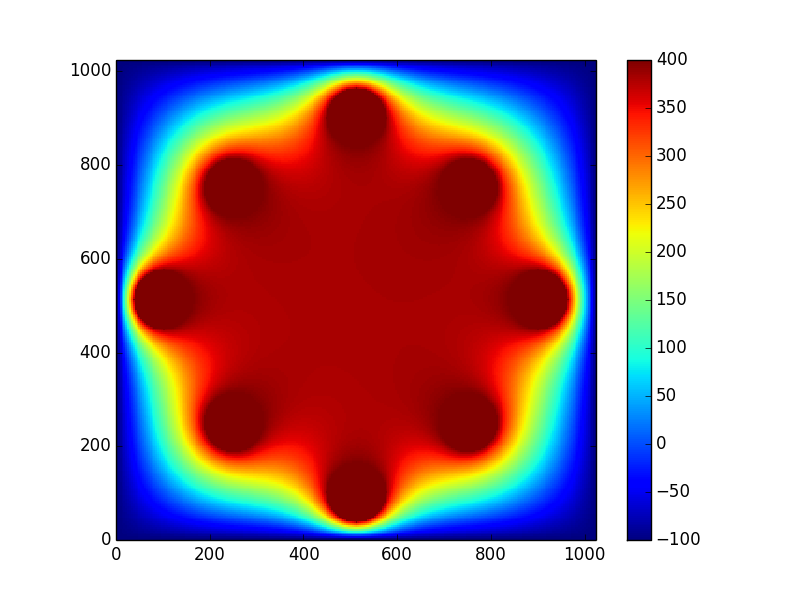
\includegraphics[scale=0.3]{imagenes/caso1_4.png} 
\caption{Granularidad: 4 - Temperatura: 382.021$^{\circ}$} 
        \end{center}
\endminipage\hfill
\minipage{0.5\textwidth}
\begin{center}
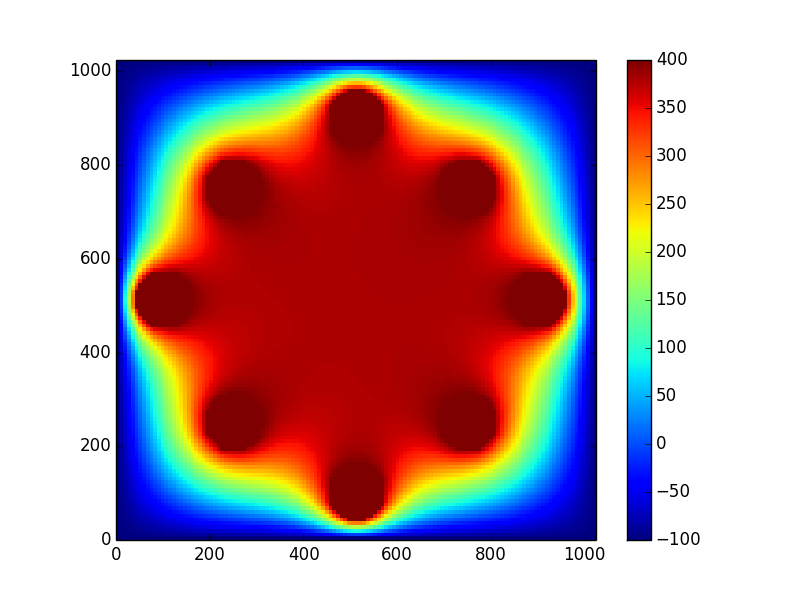
\includegraphics[scale=0.3]{imagenes/caso1_8.png} 
\caption{Granularidad: 8 - Temperatura: 380.138$^{\circ}$} 
        \end{center}
\endminipage\hfill 
\end{figure}

\begin{figure}[htb]
\minipage{0.5\textwidth}
\begin{center}
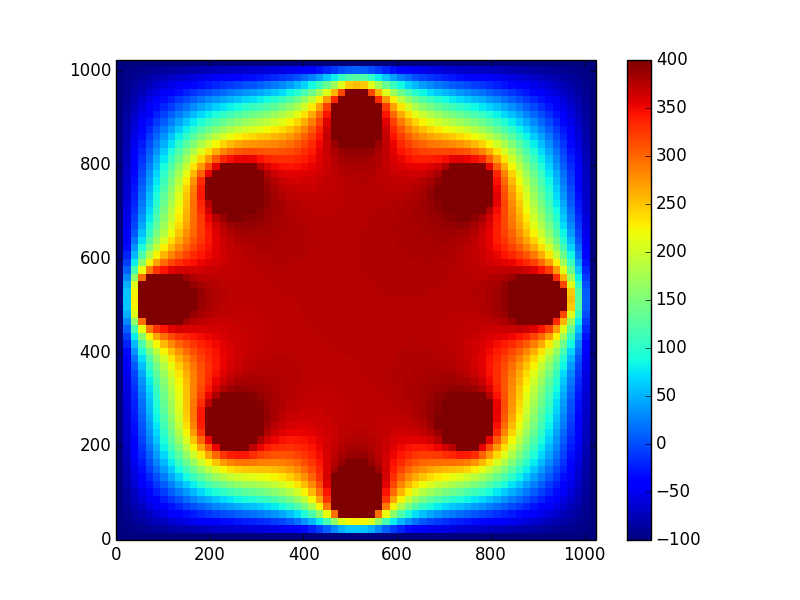
\includegraphics[scale=0.3]{imagenes/caso1_16.png} 
\caption{Granularidad: 16 - Temperatura: 375.96$^{\circ}$} 
        \end{center}
\endminipage\hfill
\minipage{0.5\textwidth}
\begin{center}
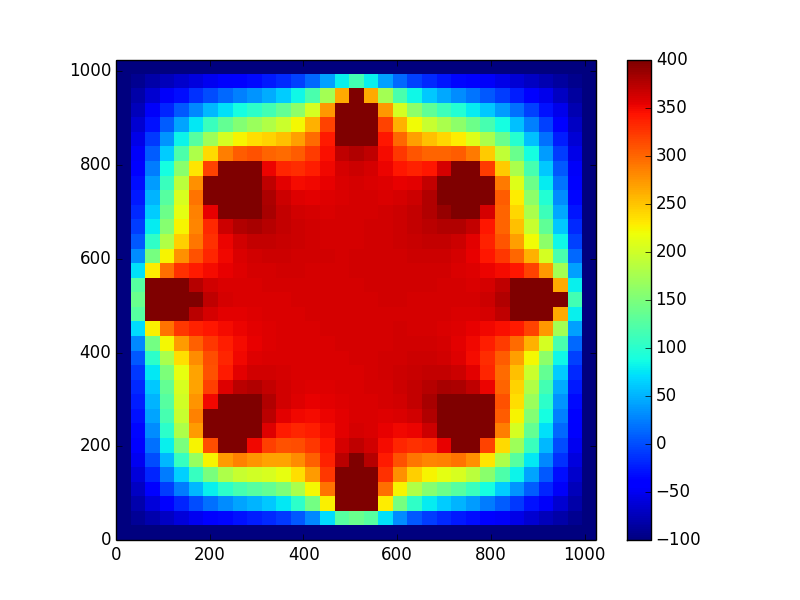
\includegraphics[scale=0.3]{imagenes/caso1_32.png} 
\caption{Granularidad: 32 - Temperatura: 362.425$^{\circ}$} 
        \end{center}
\endminipage\hfill 
\end{figure}

\begin{figure}[htb]
\minipage{0.5\textwidth}
\begin{center}
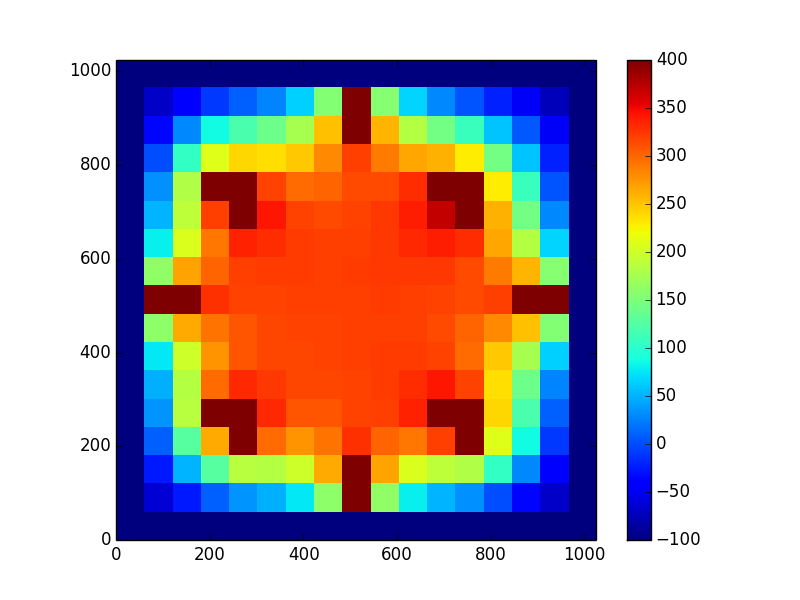
\includegraphics[scale=0.3]{imagenes/caso1_64.png} 
\caption{Granularidad: 64 - Temperatura: 321.288$^{\circ}$} 
        \end{center}
\endminipage\hfill
\minipage{0.5\textwidth}
\begin{center}
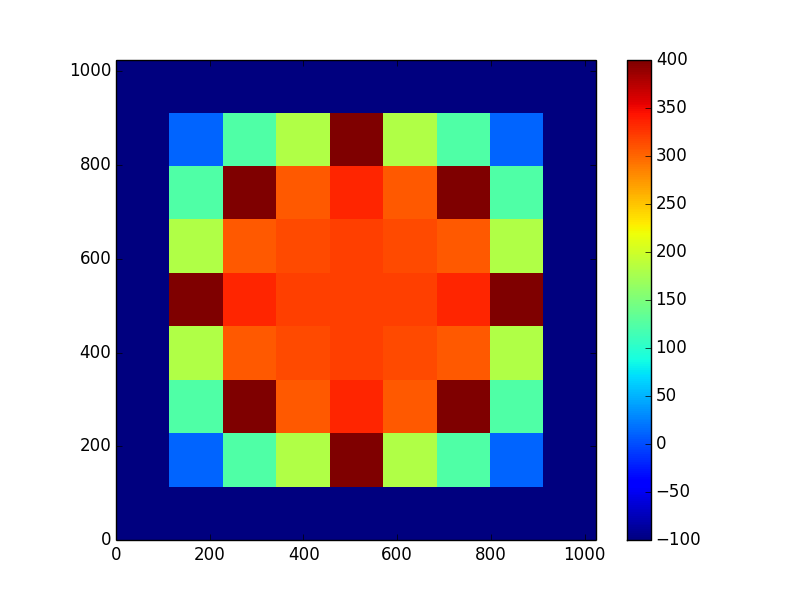
\includegraphics[scale=0.3]{imagenes/caso1_128.png} 
\caption{Granularidad: 128 - Temperatura: 268.117$^{\circ}$} 
        \end{center}
\endminipage\hfill 
\end{figure}
\newpage 
Caso 2:

\begin{figure}[htb]
\minipage{0.5\textwidth}
\begin{center}
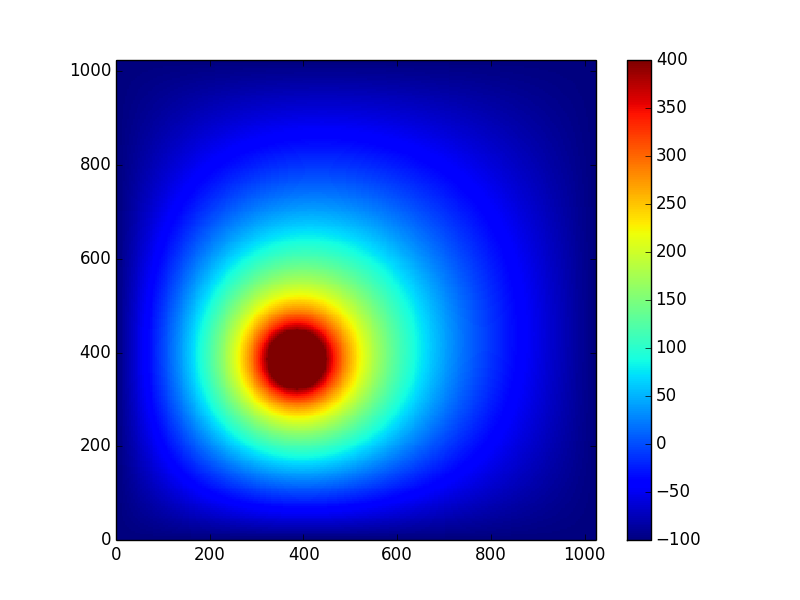
\includegraphics[scale=0.3]{imagenes/caso2_4.png} 
\caption{Granularidad: 4 - Temperatura: 166.282$^{\circ}$} 
        \end{center}
\endminipage\hfill
\minipage{0.5\textwidth}
\begin{center}
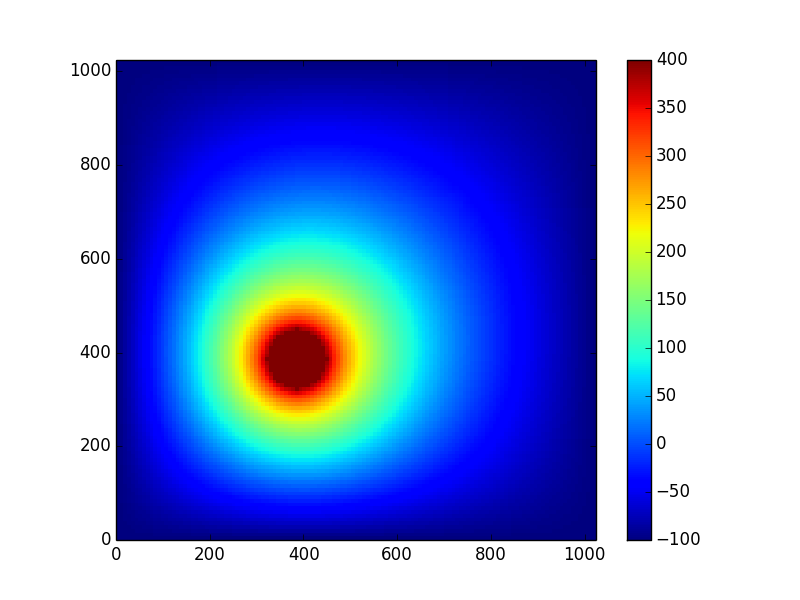
\includegraphics[scale=0.3]{imagenes/caso2_8.png} 
\caption{Granularidad: 8 - Temperatura: 163.331$^{\circ}$} 
        \end{center}
\endminipage\hfill 
\end{figure}

\begin{figure}[htb]
\minipage{0.5\textwidth}
\begin{center}
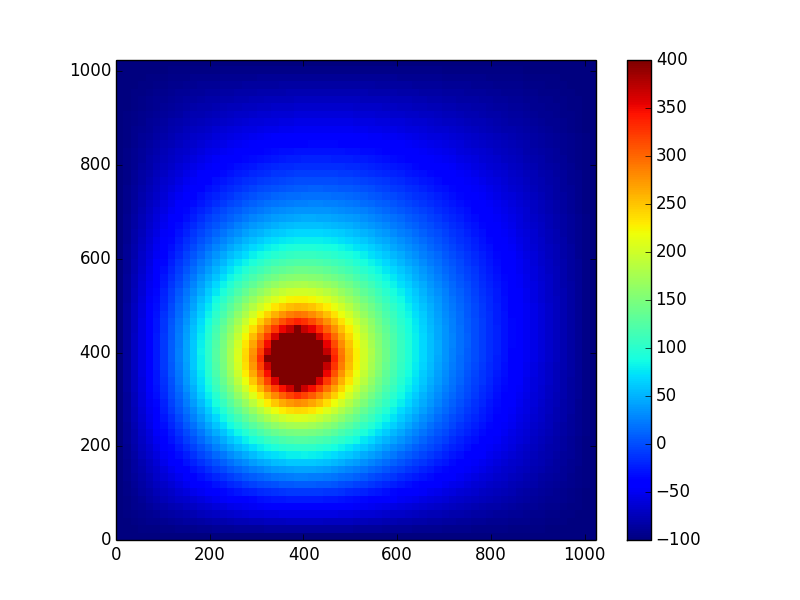
\includegraphics[scale=0.3]{imagenes/caso2_16.png} 
\caption{Granularidad: 16 - Temperatura: 158.461$^{\circ}$} 
        \end{center}
\endminipage\hfill
\minipage{0.5\textwidth}
\begin{center}
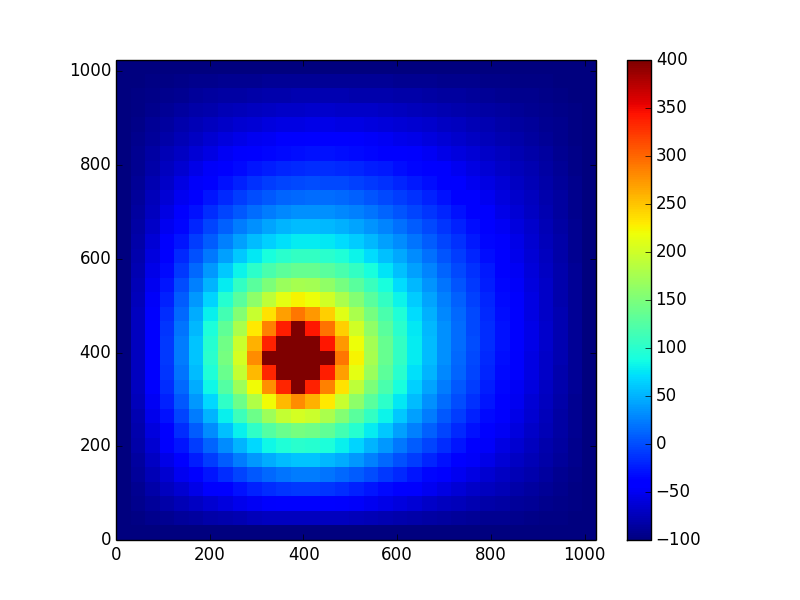
\includegraphics[scale=0.3]{imagenes/caso2_32.png} 
\caption{Granularidad: 32 - Temperatura: 153.939$^{\circ}$} 
        \end{center}
\endminipage\hfill 
\end{figure}

\begin{figure}[htb]
\minipage{0.5\textwidth}
\begin{center}
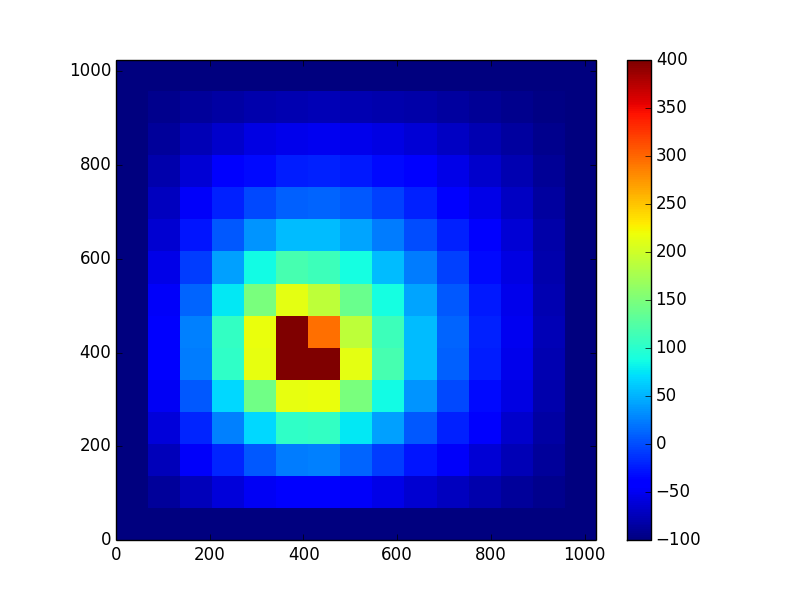
\includegraphics[scale=0.3]{imagenes/caso2_72.png} 
\caption{Granularidad: 72 - Temperatura: 138.874$^{\circ}$} 
        \end{center}
\endminipage\hfill
\minipage{0.5\textwidth}
\begin{center}
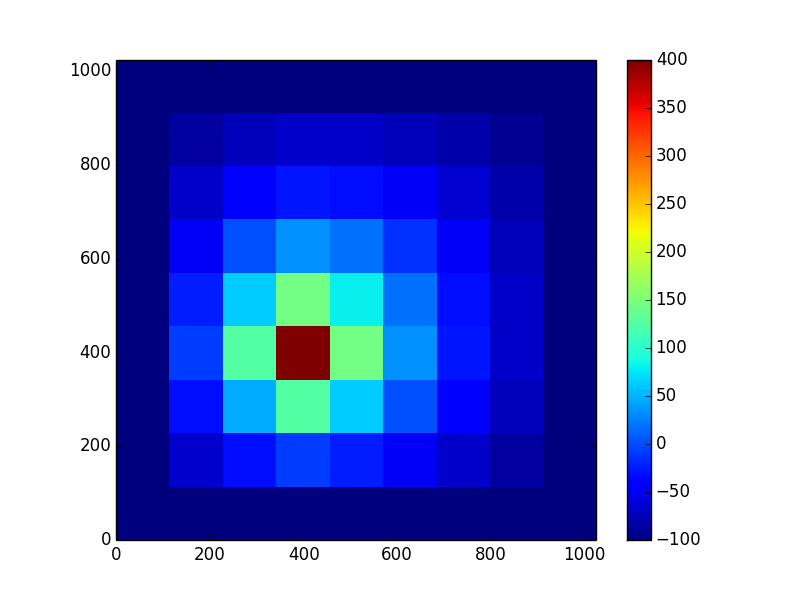
\includegraphics[scale=0.3]{imagenes/caso2_128.png} 
\caption{Granularidad: 128 - Temperatura: 81.2233$^{\circ}$} 
        \end{center}
\endminipage\hfill 
\end{figure}
\newpage
Caso 3:
\begin{figure}[htb]
\minipage{0.5\textwidth}
\begin{center}
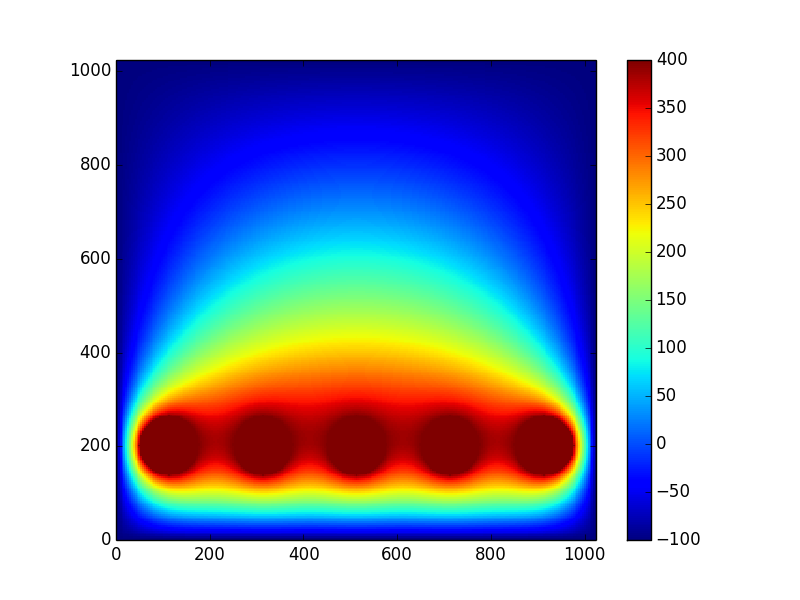
\includegraphics[scale=0.3]{imagenes/caso3_4.png} 
\caption{Granularidad: 4 - Temperatura: 154.532$^{\circ}$} 
        \end{center}
\endminipage\hfill
\minipage{0.5\textwidth}
\begin{center}
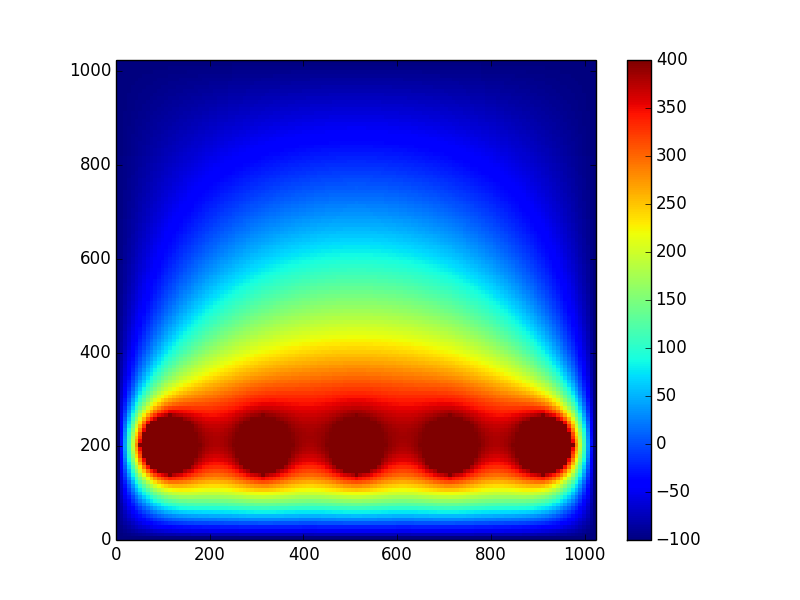
\includegraphics[scale=0.3]{imagenes/caso3_8.png} 
\caption{Granularidad: 8 - Temperatura: 153.194$^{\circ}$} 
        \end{center}
\endminipage\hfill 
\end{figure}

\begin{figure}[htb]
\minipage{0.5\textwidth}
\begin{center}
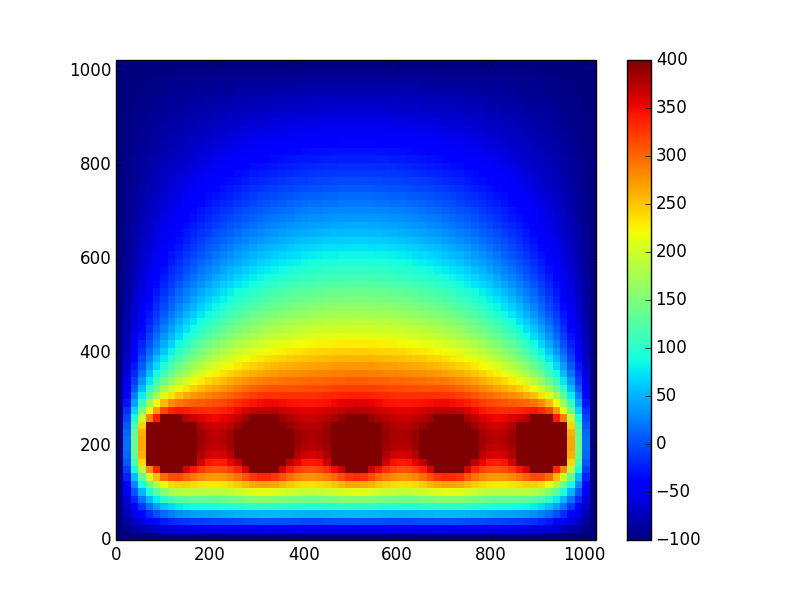
\includegraphics[scale=0.3]{imagenes/caso3_16.png} 
\caption{Granularidad: 16 - Temperatura: 150.55$^{\circ}$} 
        \end{center}
\endminipage\hfill
\minipage{0.5\textwidth}
\begin{center}
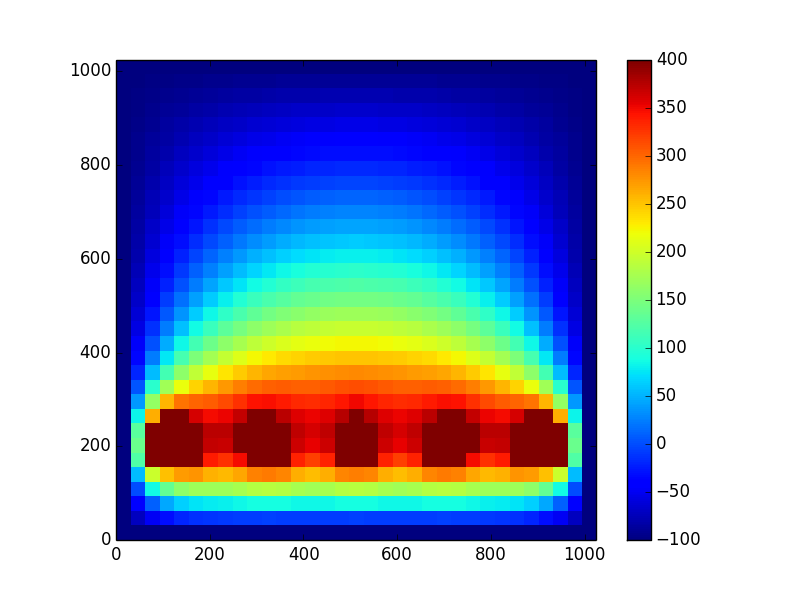
\includegraphics[scale=0.3]{imagenes/caso3_32.png} 
\caption{Granularidad: 32 - Temperatura: 146.013$^{\circ}$} 
        \end{center}
\endminipage\hfill 
\end{figure}

\begin{figure}[htb]
\minipage{0.5\textwidth}
\begin{center}
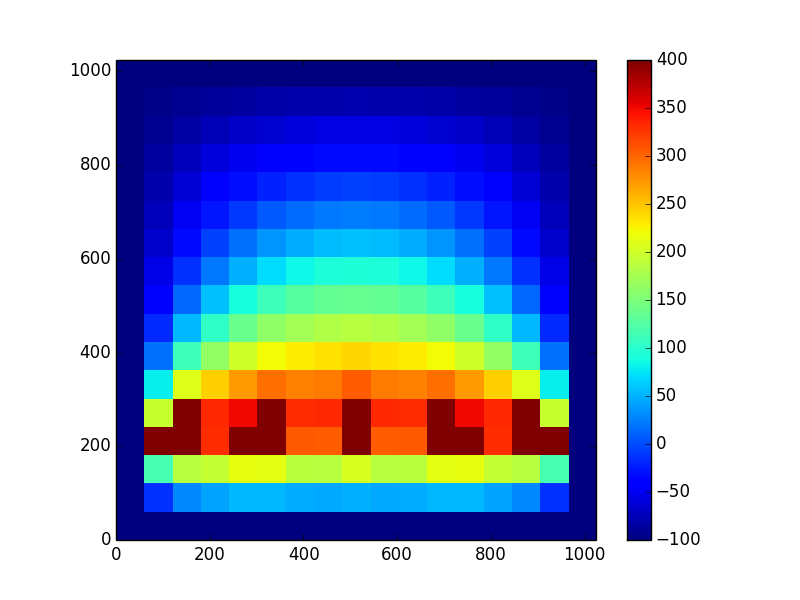
\includegraphics[scale=0.3]{imagenes/caso3_64.png} 
\caption{Granularidad: 64 - Temperatura: 137.51$^{\circ}$} 
        \end{center}
\endminipage\hfill
\minipage{0.5\textwidth}
\begin{center}
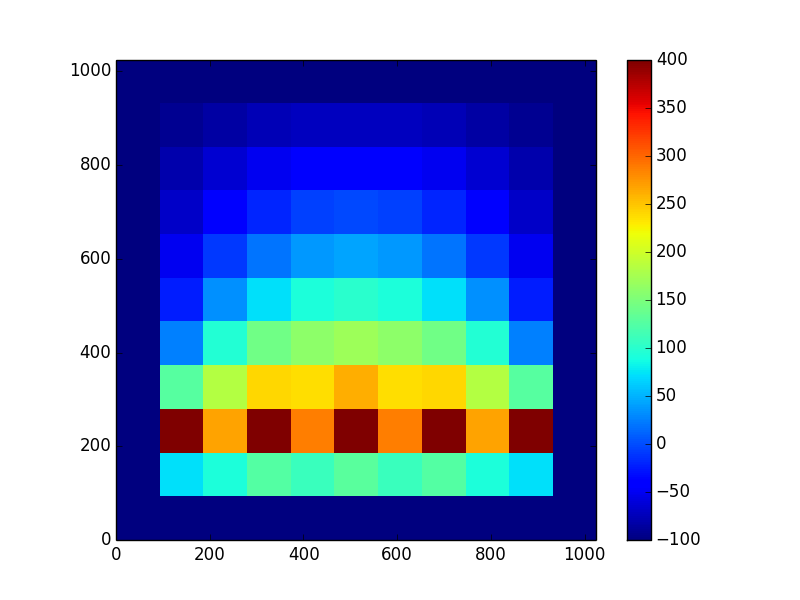
\includegraphics[scale=0.3]{imagenes/caso3_100.png} 
\caption{Granularidad: 100 - Temperatura: 100.115$^{\circ}$} 
        \end{center}
\endminipage\hfill 
\end{figure}
\newpage
\begin{figure}[htb]
\begin{center}
        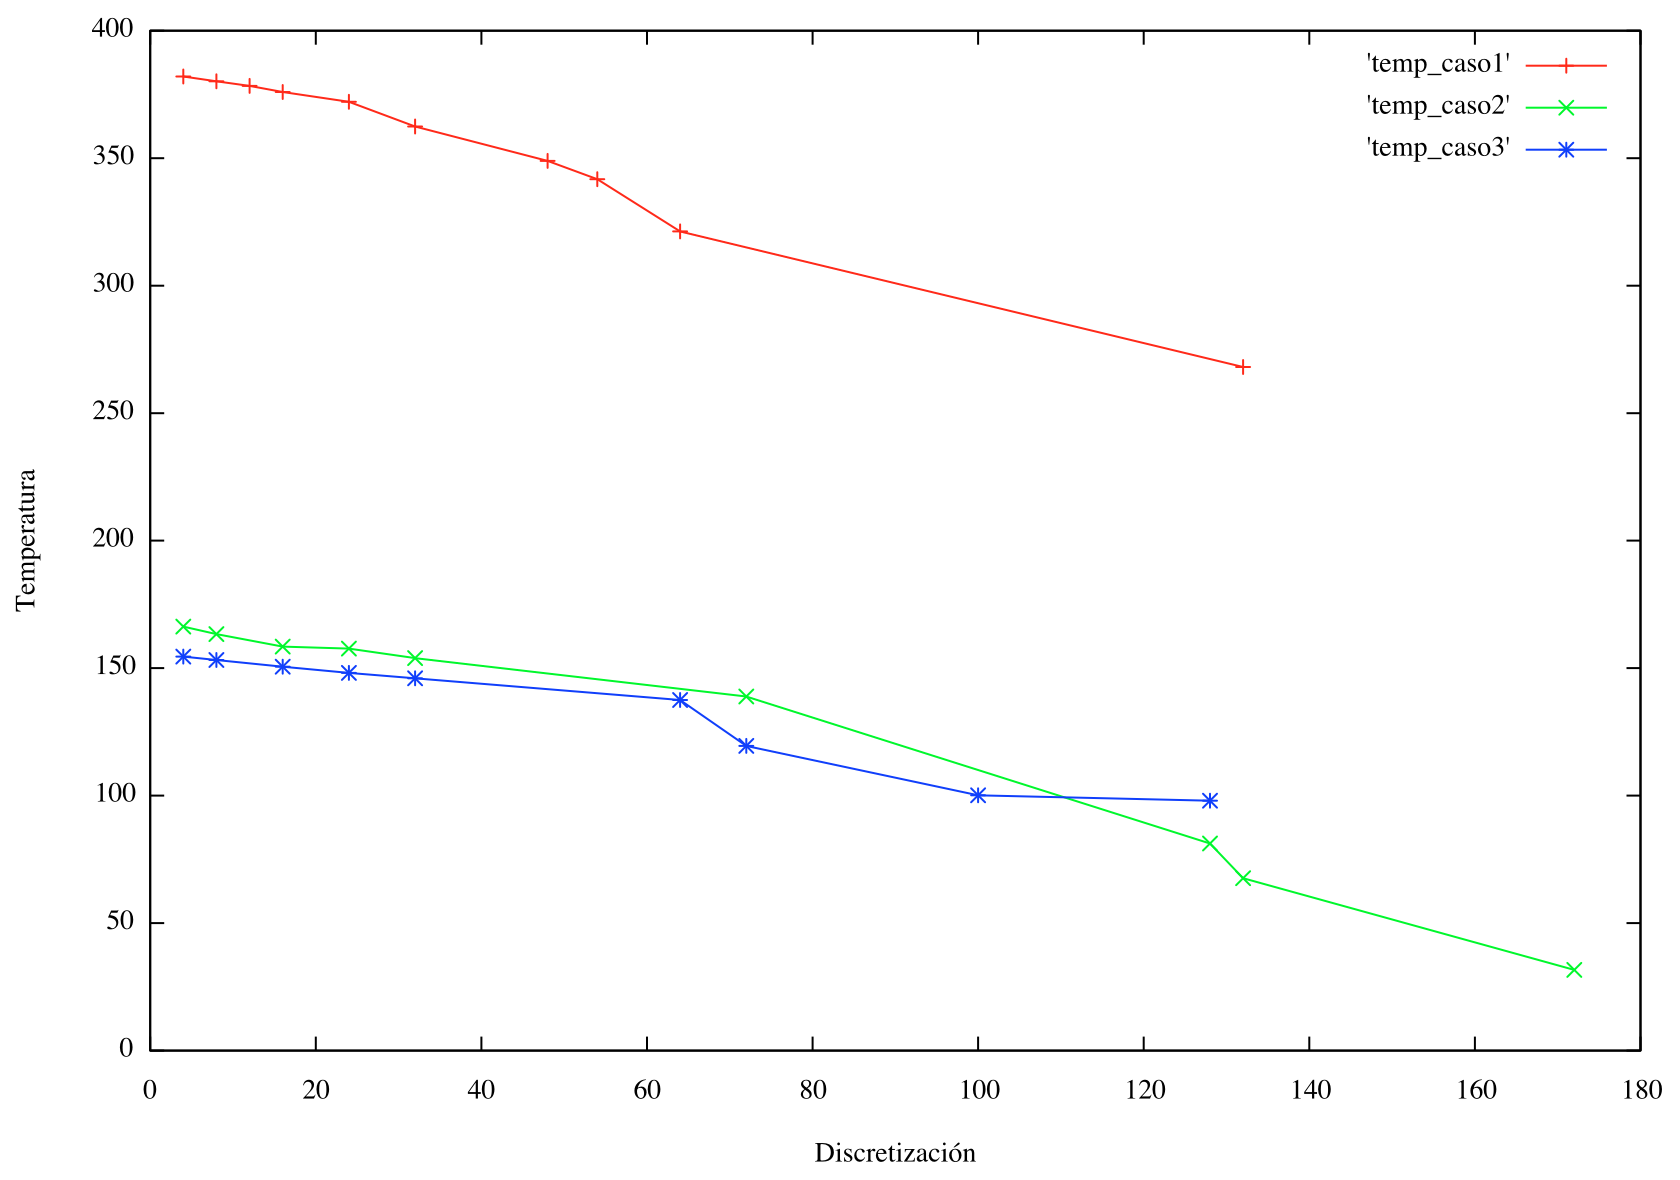
\includegraphics[scale=0.5]{imagenes/comparacion_temperatura.png}
                \caption{Comparación de temperaturas}
        \end{center}

\end{figure}

Por lo que se puede observar en los gráficos de como va fluctuando la temperatura a medida que se aumenta el valor de discretización (que provoca disminución en la granuralidad) para los 3 casos de prueba y con el ultimo gráfico comparativo, como era de esperarse, la temperatura disminuye en el punto crítico, esto es debido a que a mayor granularidad las sanguijuelas tienen mas borde en el parabrisas para transferir el calor ya que dependiendo el radio de la sanguijuela provoca que ocupe más puntos en el parabrisas. Esto último del radio se puede ver cuando en los últimos gráficos de cada caso cuando la garrulidad es minima que las sanguijuelas pasan a ocupar una posición del parabrisas.

\newpage

\subsection{Tiempo de corrida variando granularidad}

\begin{figure}[htb]
\begin{center}
        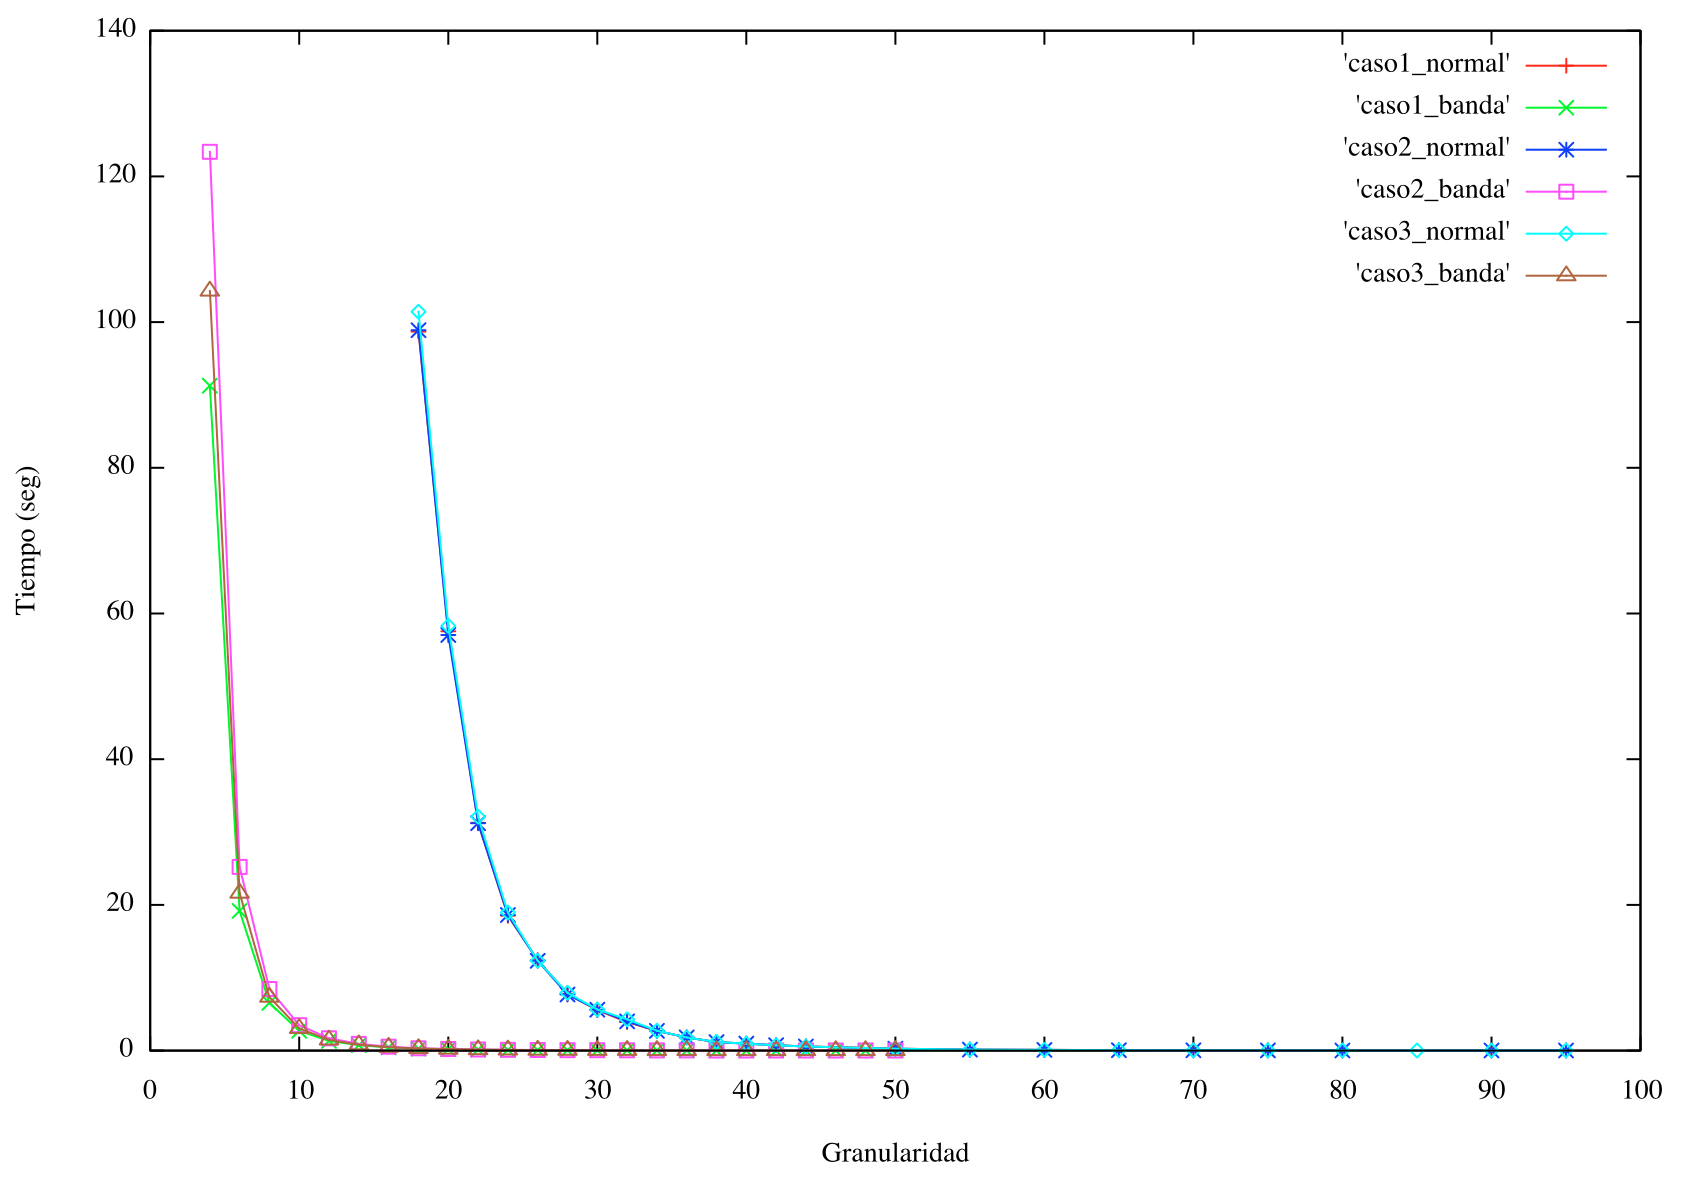
\includegraphics[scale=0.5]{imagenes/comparacion_tiempos.png}
                \caption{Comparación de tiempos}
        \end{center}

\end{figure}
\subsection{Caso básico}
\newpage
A continuación plantearemos distintos casos de parabrisas con distintas granularidades que utlizaremos durante las pruebas. 

\begin{figure}[htb]

\minipage{0.5\textwidth}
\begin{center}
       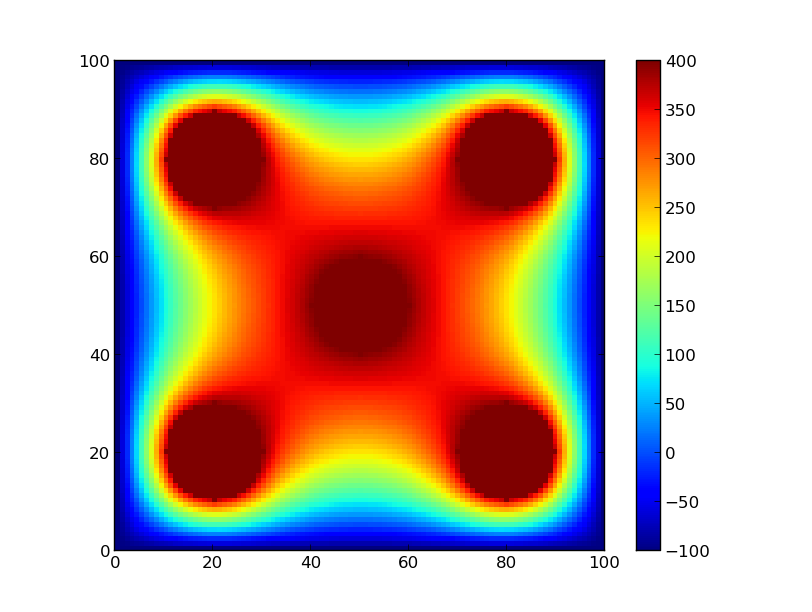
\includegraphics[scale=0.3]{imagenes/test5_gran1.png}
                \caption{Granularidad 1}
        \end{center}
\endminipage\hfill
\minipage{0.5\textwidth}
\begin{center}
        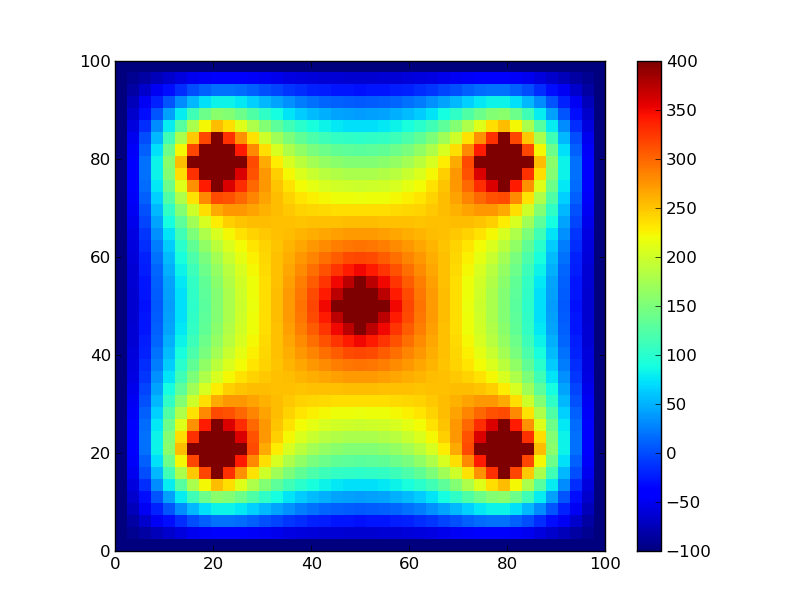
\includegraphics[scale=0.3]{imagenes/test5.png}
                \caption{Granularidad 2.5}
        \end{center}
\endminipage\hfill 
\end{figure}

\begin{figure}[!htb]
\minipage{0.5\textwidth}
\begin{center}
    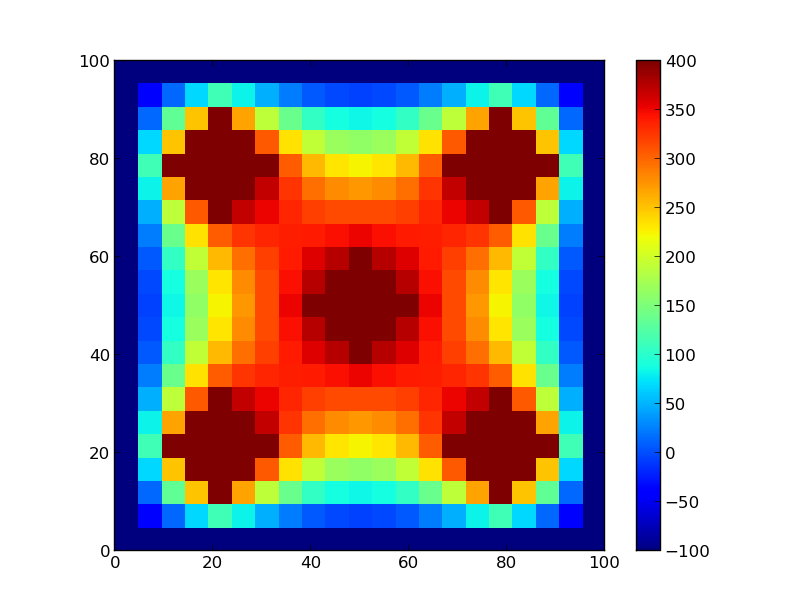
\includegraphics[scale=0.3]{imagenes/test5_gran5.png}
                \caption{Granularidad 5}
 \end{center}
\endminipage
\minipage{0.5\textwidth}
\begin{center}
   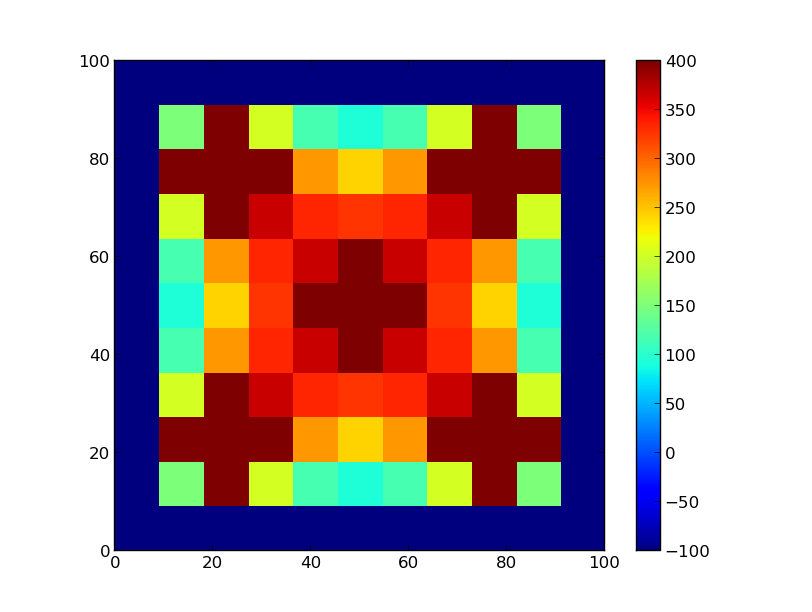
\includegraphics[scale=0.3]{imagenes/test5_gran10.png}
                \caption{Granularidad 10}
        \end{center}
\endminipage\hfill
\end{figure}
\clearpage

\subsubsection{Resultados Random}

A continuación observaremos un caso en la que la única sanguijuela que se debe eliminar es la del centro. Esta se encuentra exactamente en el punto central. Adicionalmente hay otras 4 sanguijuelas en las puntas. 
Matar a estas no soluciona nada ya que la del centro esta aplicando una temperatura constante de 400 Cº. Lo observaremos con 4 discretizaciones distintas para tener un mas amplio panorama.
\begin{figure}[htb]
\begin{center}
        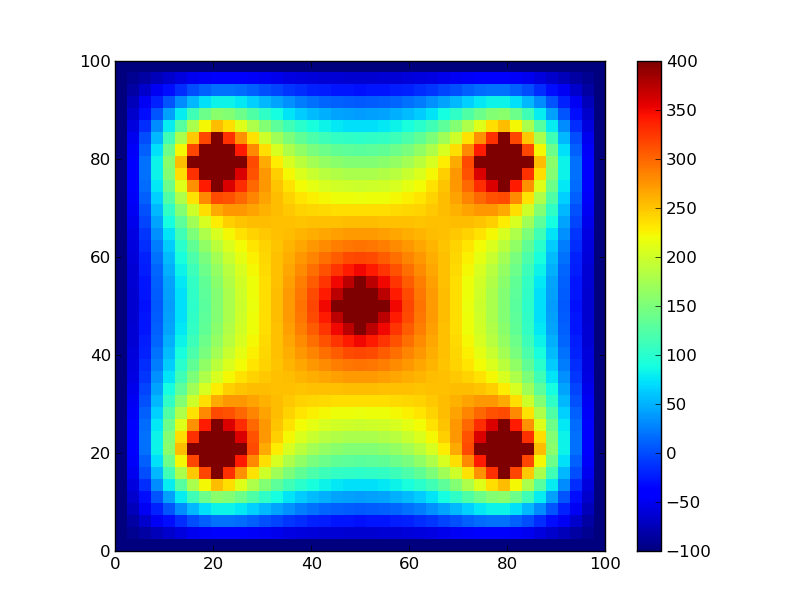
\includegraphics[scale=0.3]{imagenes/test5.png}
                \caption{Granularidad 2.5}
        \end{center}

\end{figure}

Ahora veamos que obtenemos al aplicarle distintas veces el algoritmo de solución random explicado en el desarrollo (\ref{sec:solucionRandom}).

\begin{figure}[htb]

\minipage{0.5\textwidth}
\begin{center}
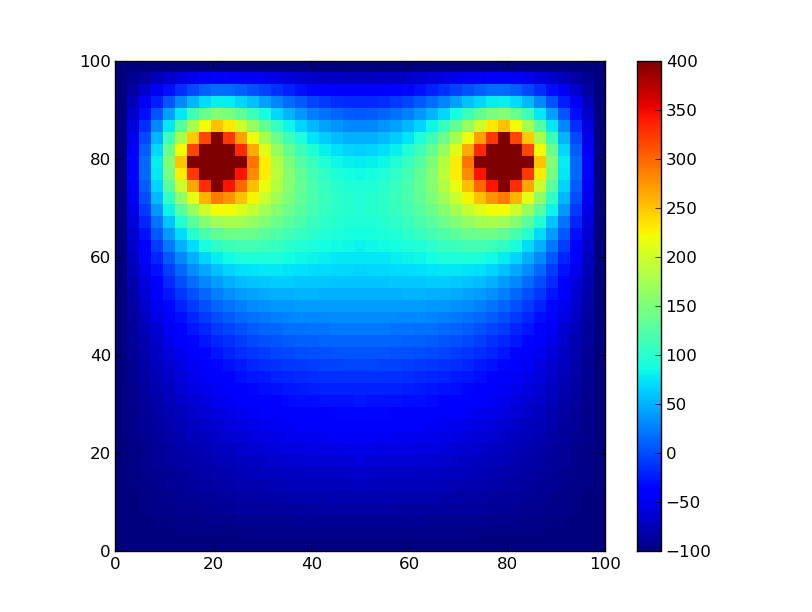
\includegraphics[scale=0.3]{imagenes/random_1.png} 
\caption{Resultado primer corrida} 
        \end{center}
\endminipage\hfill
\minipage{0.5\textwidth}
\begin{center}
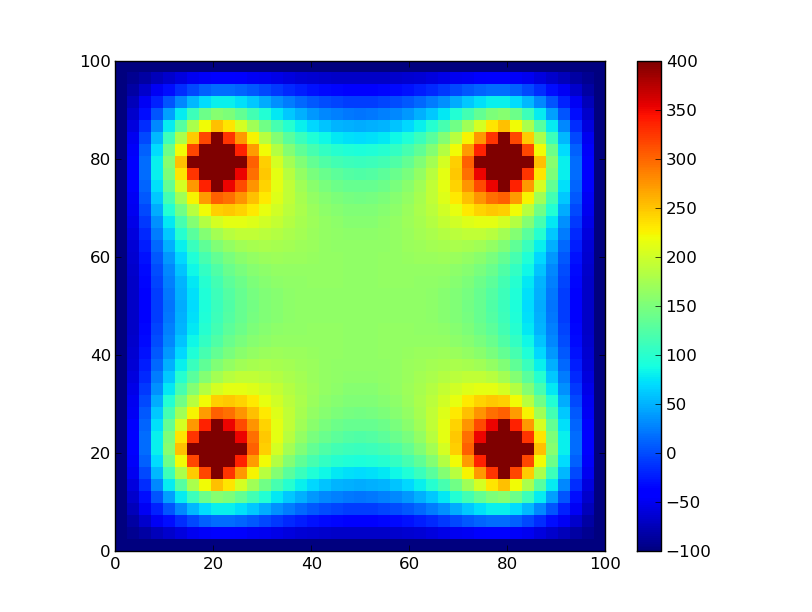
\includegraphics[scale=0.3]{imagenes/random_2.png} 
\caption{Resultado segunda corrida} 
        \end{center}
\endminipage\hfill 
\end{figure}

\begin{figure}[htb]
\begin{center}
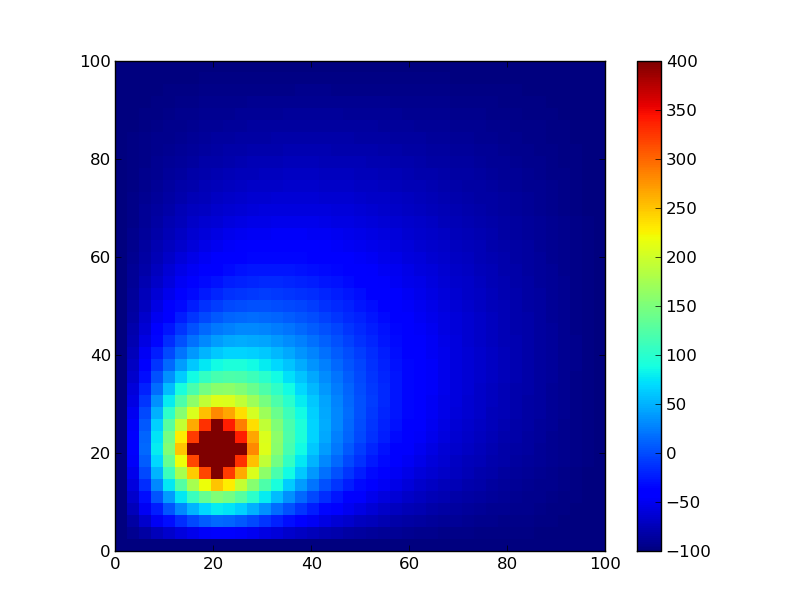
\includegraphics[scale=0.3]{imagenes/random_3.png} 
\caption{Resultado tercer corrida} 
\end{center}
\end{figure}
Como podemos observar la solución óptima (la que menos sanguijuelas elimina), es la segunda. Pero como esta solución es completamente random en la primera corrida mata 2 sanguijuelas antes de elegir 
la correcta y en la tercera 4. Sólo en la segunda elije en el primer intento la sanguijuela correcta. Se aplicó también para todas las granularidades antes mencionadas y se observó el mismo comportamiento erratico a la hora
de matar sanguijuelas. 

\clearpage


\subsubsection{Resultados Greedy}

Veamos ahora para la misma matriz como se comporta nuestro otro algoritmo. 


\begin{figure}[htb]
\begin{center}
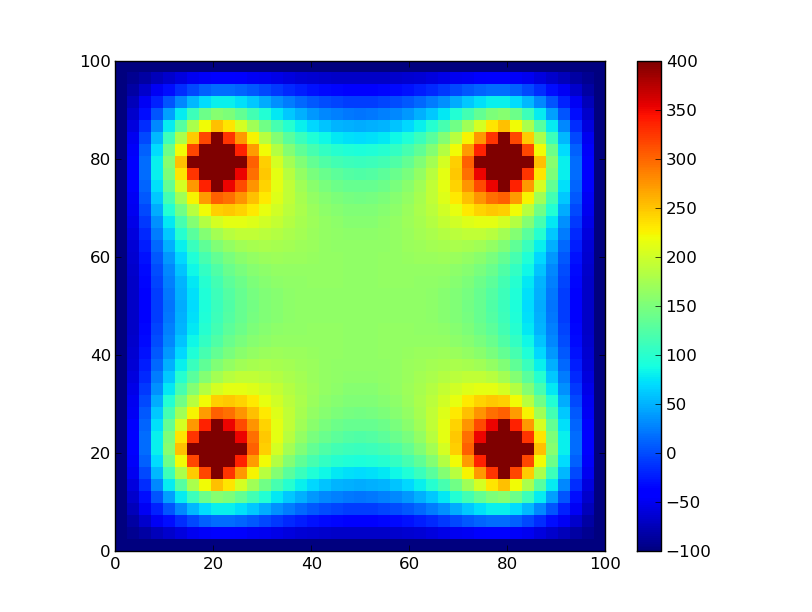
\includegraphics[scale=0.40]{imagenes/random_2.png} 
\caption{Resultado corrida con greedy} 
\end{center}
\end{figure}


En todas las corridas obtuvimos el mismo resultado y demoraron lo mismo. Era de esperarse, ya que efectivamente en este caso, la sanguijuela a eliminar era la del medio.
\newpage
\subsection{Resultados Banda VS Gaussiano}
Veamos ahora que realmente valió la pena la mejora al saber que era matriz banda en cuanto a tiempos en comparación con la eliminación gaussiana.
Anotamos que agregar un análisis de resultados no vale la pena ya que son el mismo

\begin{figure}[htb]
\begin{center}
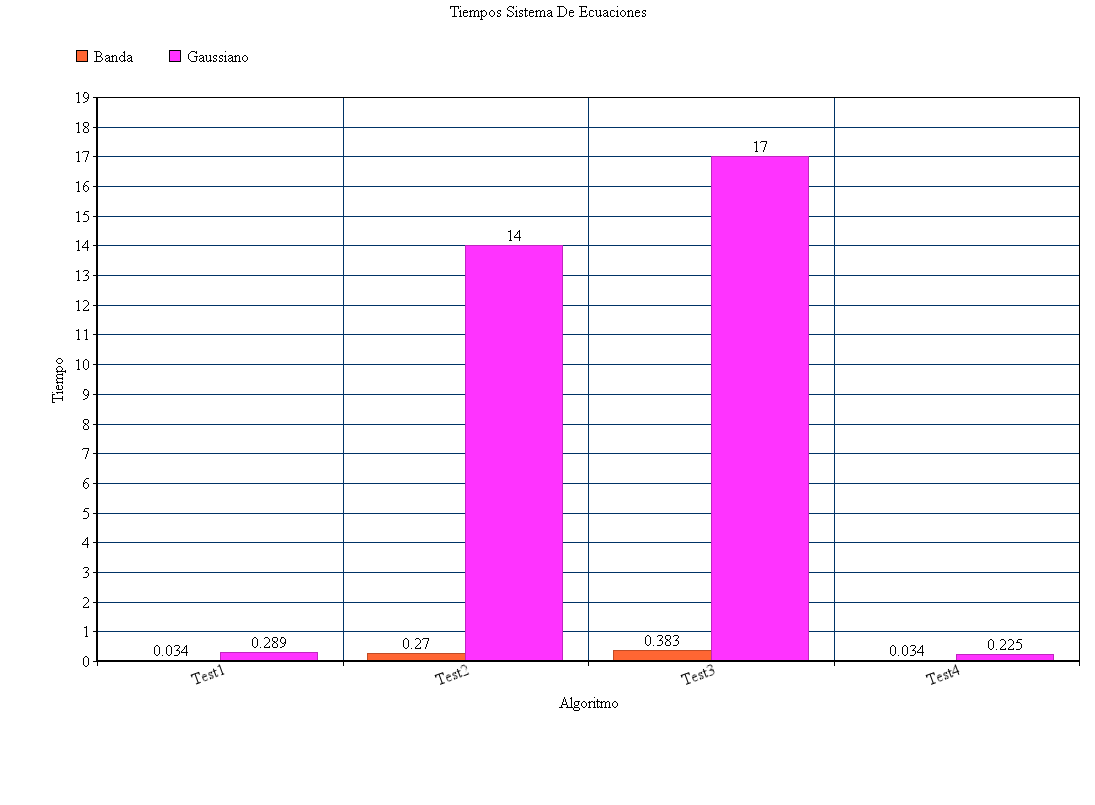
\includegraphics[scale=0.50]{imagenes/tiemposGaussVsBanda.png} 
\caption{Gauss VS Banda} 
\end{center}
\end{figure}
\clearpage
\subsection{Caso solución no es el mas cercano}

A continuación analizaremos un caso en el cual se debe eliminar una sanguijuela que no es la más cercana para efectivamente poder reducir la temperatura en punto crítico. Lo Chequearemos tanto para Greedy como para el Random, haciendo 3 corridas para este último ya que sabemos que su comportamiento es fluctuoso.
Los datos exactos de este test son:\\
Medidas: 100 x 100 \\* 
discretización:1 \\* 
radio: 0.9 \\* 
tempreratura sanguijuelas:450 \\* 
Posiciónes sanguijuelas:(49, 38);(57, 60);(57, 37);(39, 37);(36, 47) \\* 
\begin{figure}[htb]
\begin{center}
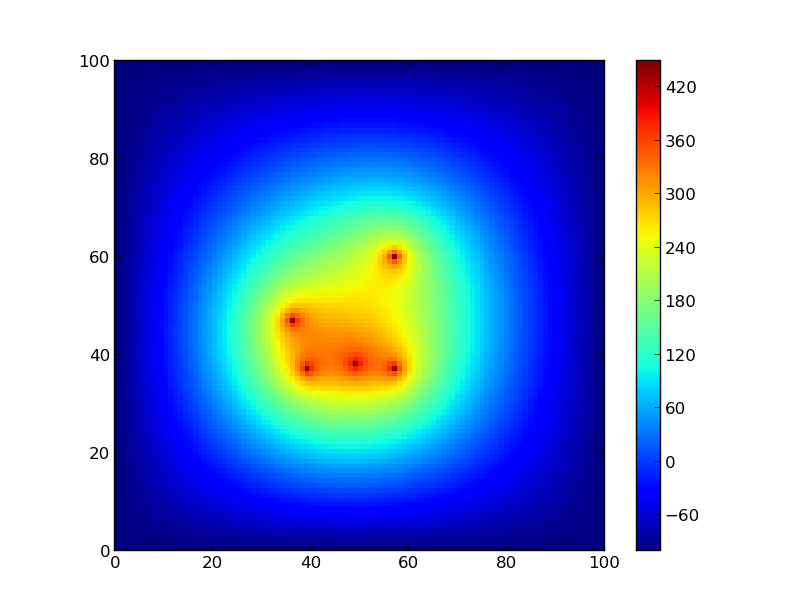
\includegraphics[scale=0.40]{imagenes/test6.png} 
\caption{Parabrisas granularidad 1} 
\end{center}
\end{figure}

Como podemos observar en las imágenes que están debajo, la solución greedy no es la óptima ya que mató a una sanguijuela extra. Esto es debido a que la principal radiación de calor era producida por el conjunto de 
sanguijuelas que están debajo del punto crítico y no por la mas cercana. Si eliminamos la sanguijuela central de aquel conjunto la radiación de calor emitida por él disminuye drásticamente en el punto crítico produciendo 
que la temperatura esté por debajo de los 235 grados sin necesidad de eliminar a las mas cercana. 

\begin{figure}[htb]
\minipage{0.5\textwidth}
\begin{center}
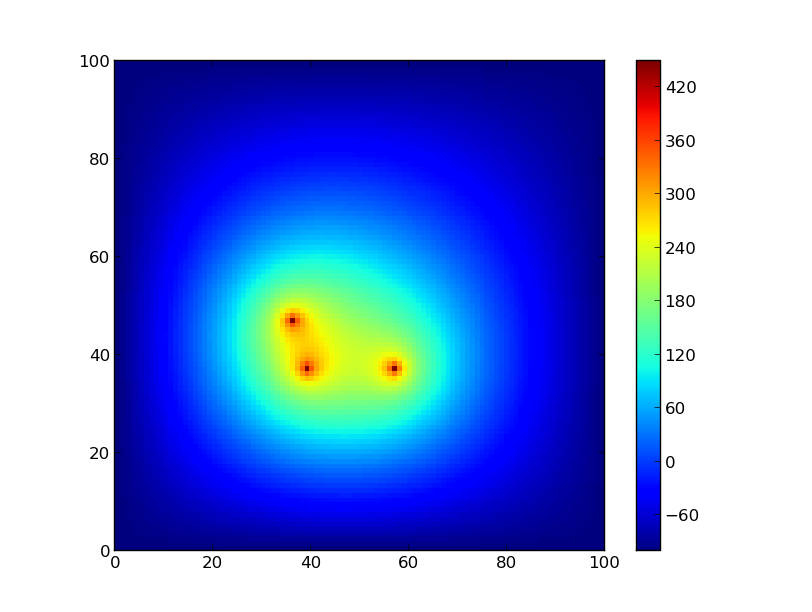
\includegraphics[scale=0.40]{imagenes/test6_greedy.png} 
\caption{Solución Greedy} 

        \end{center}
\endminipage\hfill
\minipage{0.5\textwidth}
\begin{center}
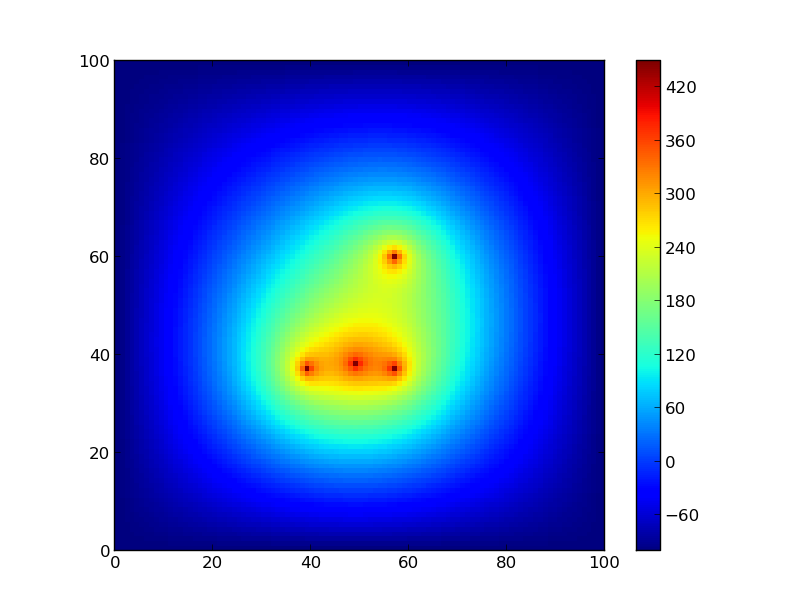
\includegraphics[scale=0.40]{imagenes/test6_random.png} 
\caption{Solución Random 1} 
        \end{center}
\endminipage\hfill 
\end{figure}
\clearpage
\begin{figure}[htb]
\minipage{0.5\textwidth}
\begin{center}
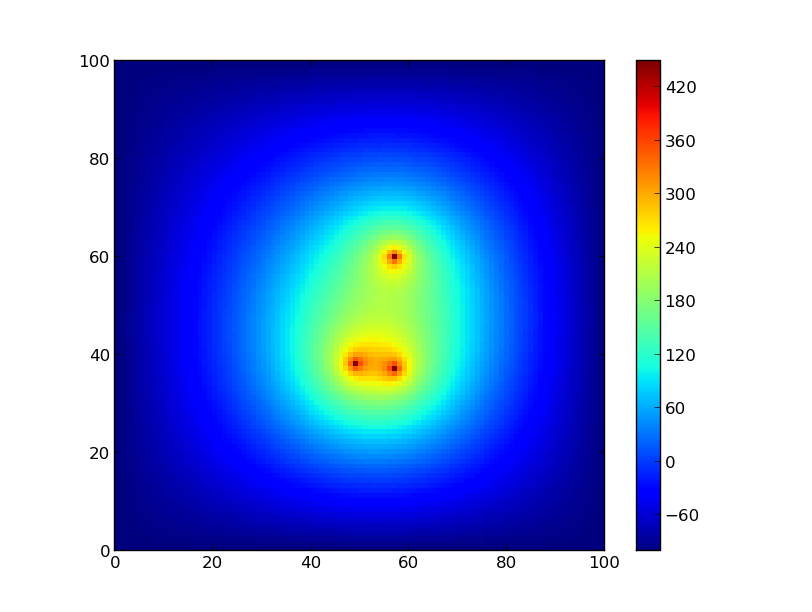
\includegraphics[scale=0.40]{imagenes/test6_random_2.png} 
\caption{Solución random 2} 
        \end{center}
\endminipage\hfill 
\minipage{0.5\textwidth}
\begin{center}
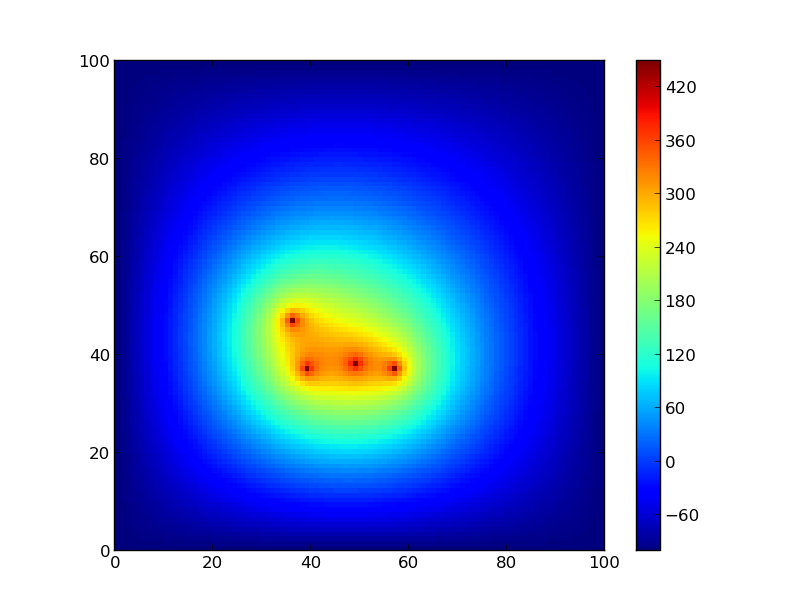
\includegraphics[scale=0.40]{imagenes/test6_random_3.png} 
\caption{Solución random 3} 
        \end{center}
\endminipage\hfill 
\end{figure}


El greedy mató primero a la sanguijuela de la posición (49,38) ya que era la mas cercana. Sin embargo si mataba primero la (57,60) la temperatura en el punto crítico disminuía lo suficiente. Esto pudimos corroborarlo al correr el test nuevamente sin esta última sangijuela y comprobando que tanto el greedy como random no mataban ninguna sangijuela ya que el punto crítica estaba por debajo de 235 grados celcius.
El random por otro lado nos dió 3 resultados distintos de los cuales dos son válidos. Cabe destacar sin embargo que el erroneo nos lo devolvió 2 veces, por lo que podemos decir que tuvo un 50\% de efectividad. 

\subsubsection{Variando la granularidad}

Como vimos anteriormente, la temperatura en el punto crítico varía según la granularidad que le demos. Veamos entonces que pasa si aumentamos la granularidad (H = 0.8 en vez de 1).

\begin{figure}[htb]
\minipage{0.5\textwidth}
\begin{center}
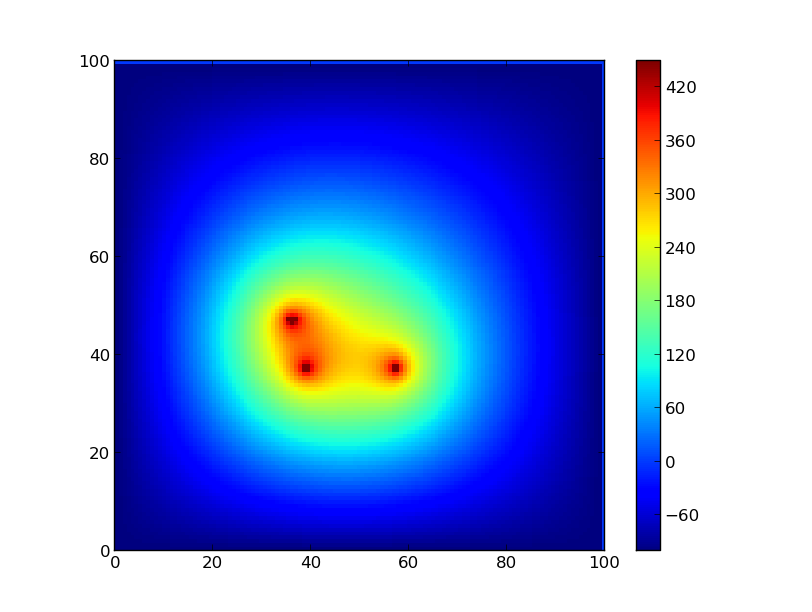
\includegraphics[scale=0.40]{imagenes/test6_g08_greedy.png} 
\caption{Solución Greedy} 

        \end{center}
\endminipage\hfill
\minipage{0.5\textwidth}
\begin{center}
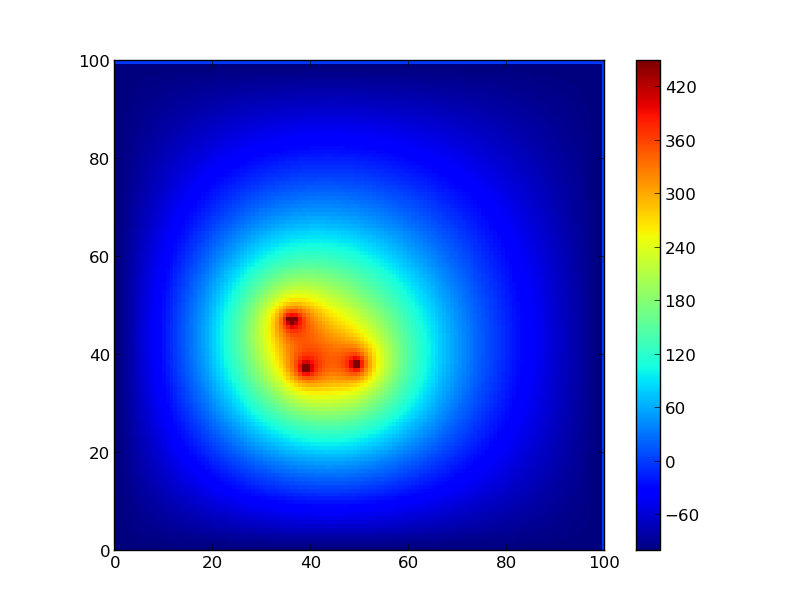
\includegraphics[scale=0.40]{imagenes/test6_g08_random.png} 
\caption{Solución Random 1} 
        \end{center}
\endminipage\hfill 
\end{figure}
\clearpage
\begin{figure}[htb]
\minipage{0.5\textwidth}
\begin{center}
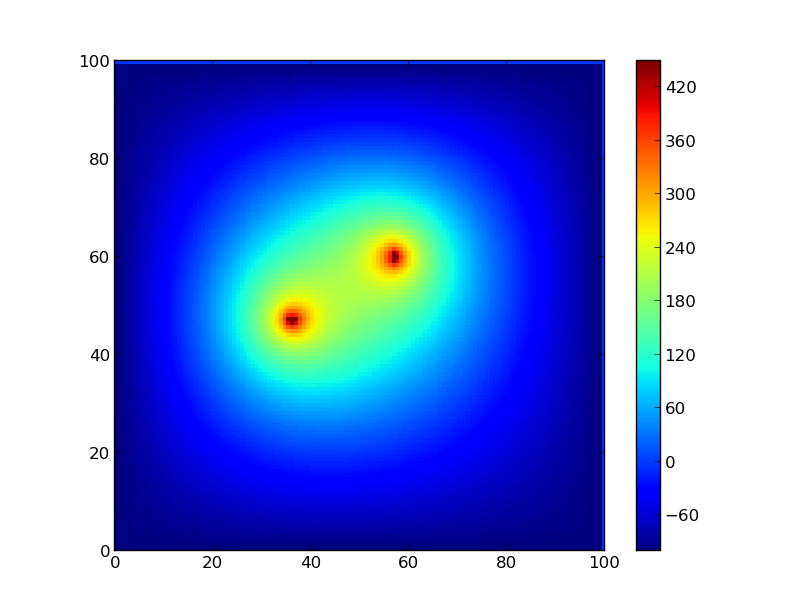
\includegraphics[scale=0.40]{imagenes/test6_g08_random_2.png} 
\caption{Solución Random 2} 

        \end{center}
\endminipage\hfill
\minipage{0.5\textwidth}
\begin{center}
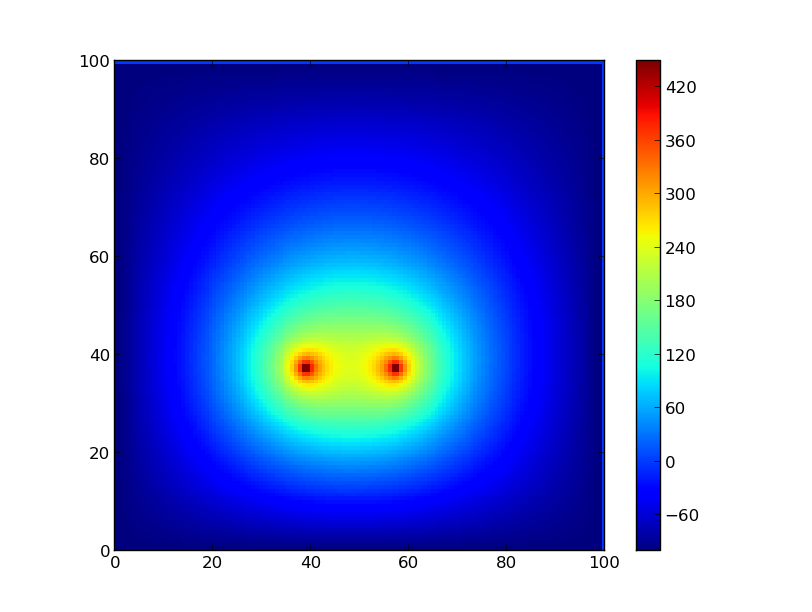
\includegraphics[scale=0.40]{imagenes/test6_g08_random_3.png} 
\caption{Solución Random 3} 
        \end{center}
\endminipage\hfill 
\end{figure}

Como le aumentamos la granularidad aumentó la temperatura del punto central de tal forma que provocó que tampoco bastase eliminando una sola sangijuela, obteniendo así la misma cantidad de sangijuelas tanto en al solución real como en la greedy. El Random esta vez devolvió un sólo resultado correcto ya que los otros dos mataron sanguijuelas de más.
